Los resultados se muestran de modo que se va aumentando el grado de las modifcaciones. Comenzamos con solo el cambio en metaheurística, seguido del cambio en la función de fitness, posteriormente se considera la extensión de vecindad planteada y por último el cambio de representación. El orden es el siguiente:
\begin{enumerate}
    \item ILS sin modificaciones
    \item ILS con diferentes funciones de fitness 
    \item ILS con extensión de vecindad
    \item ILS con la representación propuesta
\end{enumerate}
\section{ILS con vecindad N7}
A continuación se muestran los resultados de únicamente cambiar la metaheurística. Estos resultados sirven como una base para determinar si las modificaciones posteriores resultan en mejoras apreciables.

A continuación se muestran los resultados de manera gráfica para facilitar su visualización. Los resultados detallados se encuentran en el apéndice \ref{app:resn7ils}. Para cada instancia se muestra la mediana del error relativo de los resultados con respecto a los mejores resultados reportados en la literatura mostrados en el ápendice \ref{tab:sota}. 

\begin{figure}[H]
    \begin{subfigure}{\textwidth}
        \centering
        %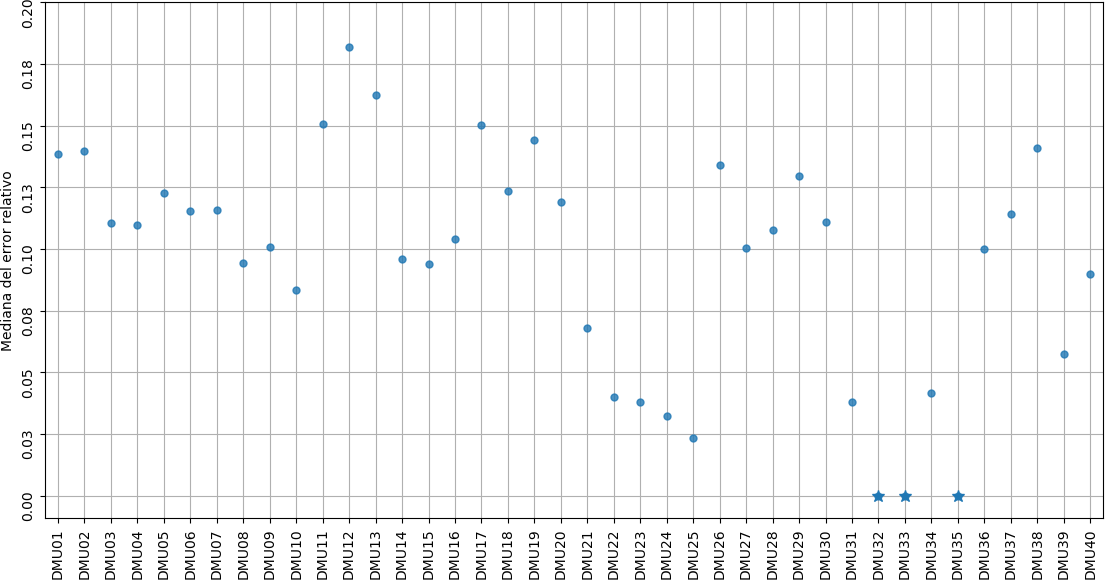
\includegraphics[height=.78\textwidth,width=.95\textheight,angle=270]{Imagenes/resn7ils1.png}
        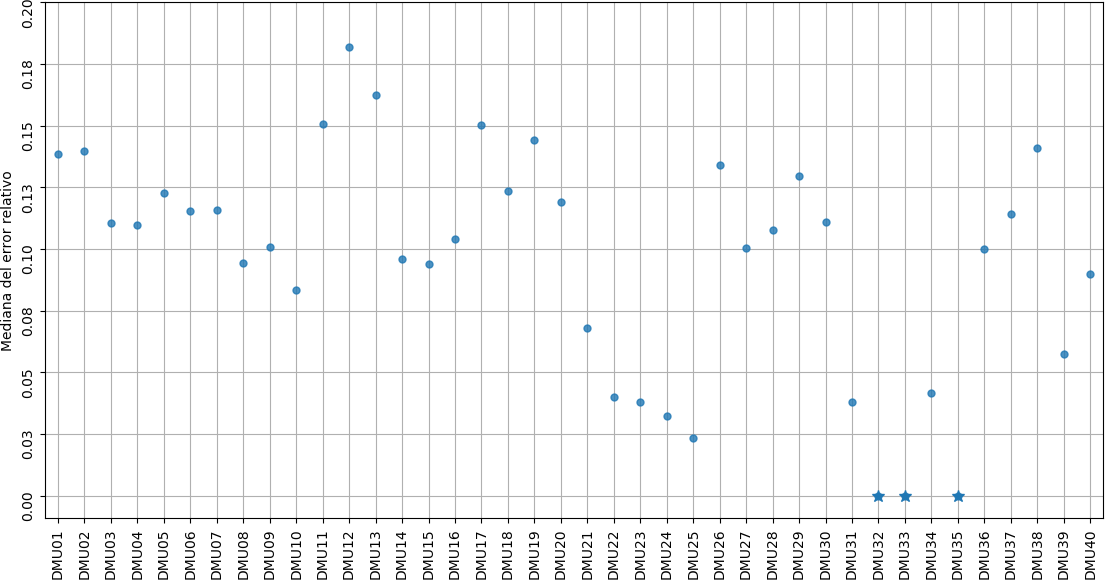
\includegraphics[scale=.65]{Imagenes/resn7ils1.png}
        \caption{Resultados para las instancias \textbf{DMU01-40}}
    \end{subfigure}
\end{figure}
\begin{figure}[H]\ContinuedFloat
    \begin{subfigure}{\textwidth}
        \centering
        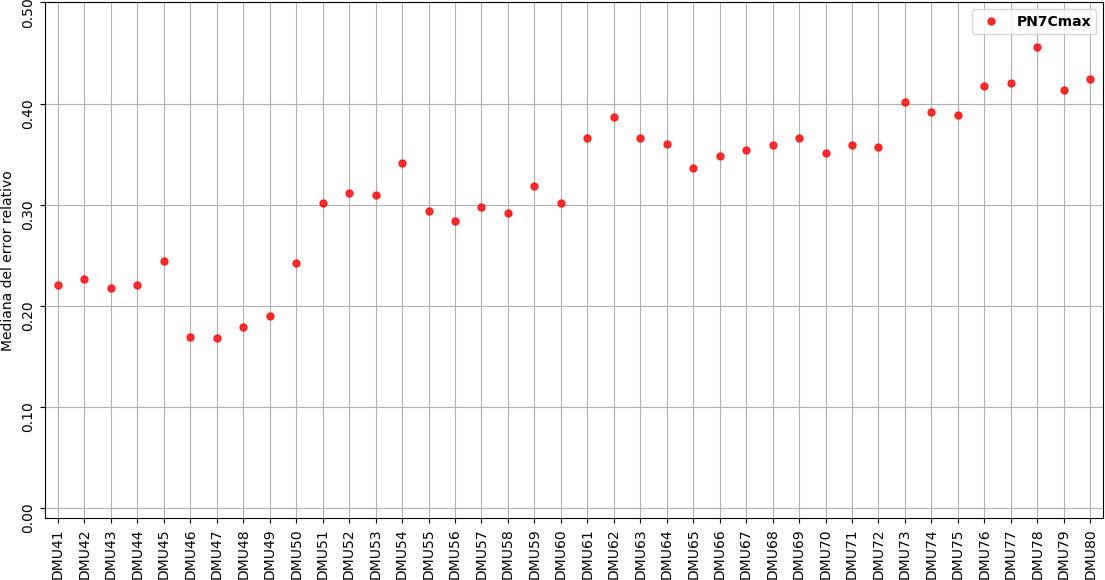
\includegraphics[scale=.65]{Imagenes/resn7ils2.png}
        \caption{Resultados para las instancias \textbf{DMU41-80}}
    \end{subfigure}
    \caption{Resultados para la propuesta más simple. Se marcan los casos en los que se llegó a la mejor solución conocida.}
\end{figure}
% grafica normalizando

\section{Función de fitness}

Para comparar los resultados obtenidos de las características propuestas para agregar al makespan en la función objetivo, se comparan por pares los conjuntos de resultados obtenidos para cada instancia. Para determinar si los conjuntos de resultados muestran diferencias estadísticamente significativas se utiliza la prueba de Wilcoxon con un nivel de significancia de $0.01$. 

Para determinar cuál es la función de fitness que obtiene mejores resultados las modificaciones a la función de fitness se comparan a pares. Si se encuentra que la diferencia entre dos modificaciones es estadísticamente significativa, se le suma un punto a la ganadora y se le resta uno a la perdedora. La función de fitness se obtiene al construir la dupla formada por el makespan y la característica en ese orden.

Los resultados para las propuestas mostradas en \ref{prop:fitness} pueden verse de manera condensada en la siguiente figura. El cuadro $(i,j)$ muestra el número de veces que $i$ fue mejor que $j$.\\
Todas las pruebas se realizaron con la vencindad N7. Se muestra también una tupla construida con las características que obtuvieron mejores resultados. Estas características se ordenan de acuerdo a su número de comparaciones ganadas totales .
\begin{figure}[H]
    \centering
    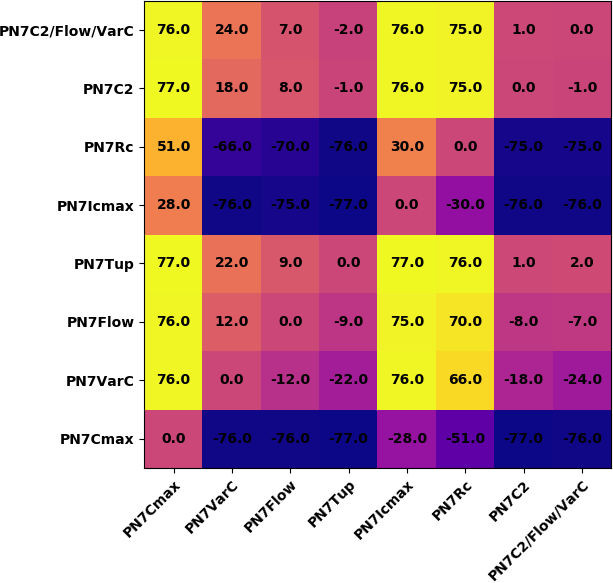
\includegraphics[scale=.8]{Imagenes/fitnesscomp.png}
    \caption{Condensado de los resultados para las modificaciones a la función de fitness. }
\end{figure}

Los mejores resultados se obtienen al construir la tupla mencionada previamente por lo que de ahora en adelante la función de fitness queda fija de esta manera y en los resultados subsecuentes solo se considera este caso. Los resultados detallados para este caso se muestran en el ápendice \ref{app:n7tuple}

\section{Extensión a vecindad N7}
Los resultados para la extensión que considera movimientos con espacios de inactividad de las máquinas se comparan con el mejor mostrado en la sección pasada. A continuación se muestra una figura en donde se comparan estos métodos de la forma que se planteó en la sección pasada.

\begin{figure}[H]
    \centering
    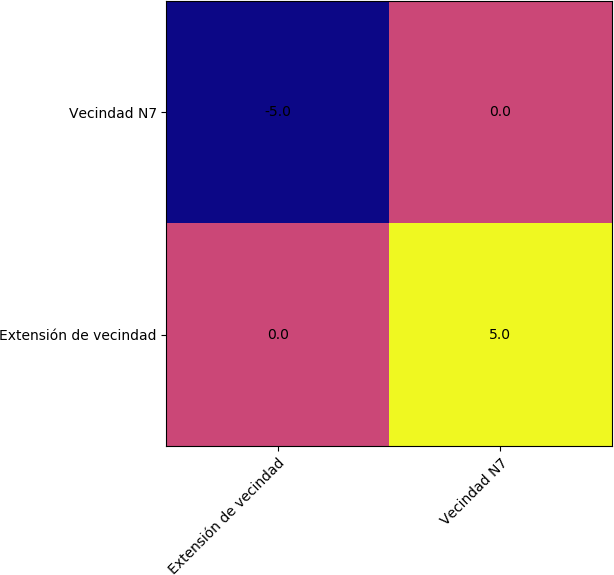
\includegraphics[scale=.7]{Imagenes/n8vsn7.png}
    \caption{Resultados de la comparación}
\end{figure}

También se muestra de manera gráfica los resultados para todas las instancias. En la siguiente figura se muestra se muestra la mediana del error relativo para cada método e instancia.  Los resultados detallados para la extensión propuesta se encuentran en el ápendice \ref{app:resn8tuple}.

\begin{figure}[H]
    \begin{subfigure}{\textwidth}
        \centering
        %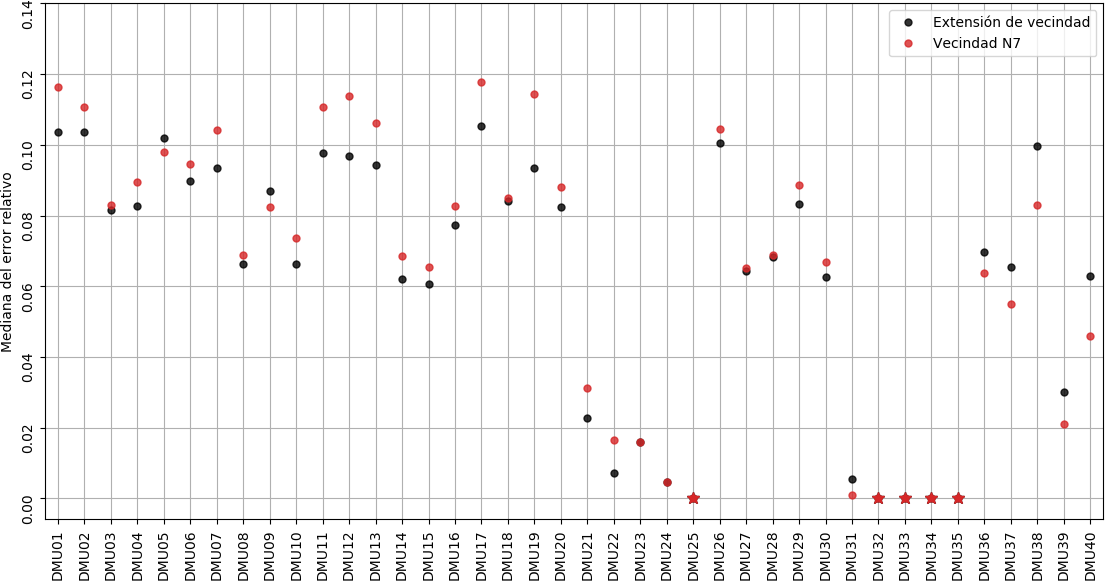
\includegraphics[height=.78\textwidth,width=.95\textheight,angle=270]{Imagenes/n8vsn7err1.png}
        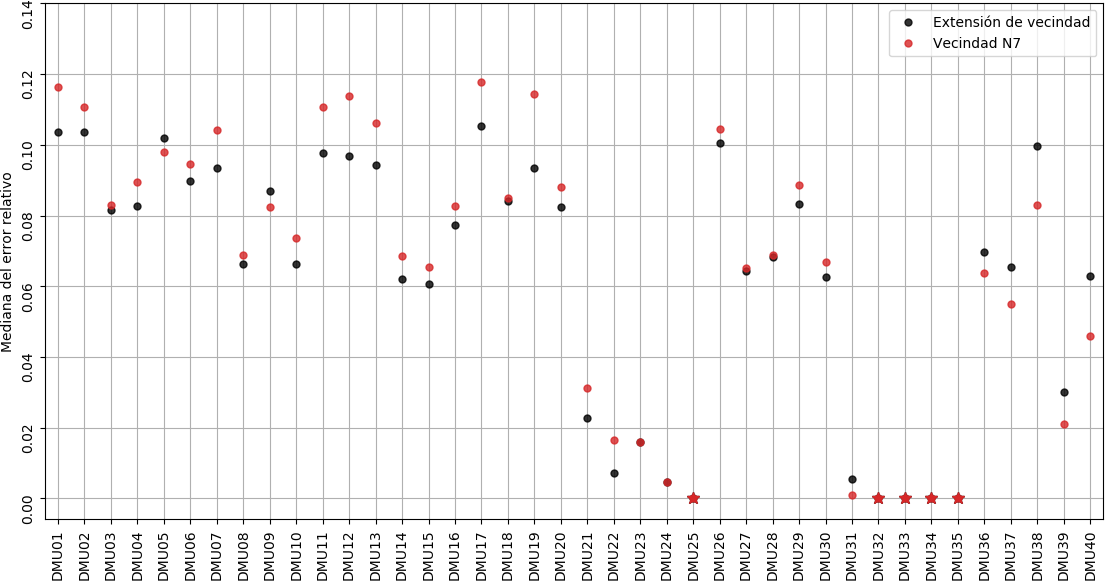
\includegraphics[scale=.6]{Imagenes/n8vsn7err1.png}
        \caption{Resultados para las instancias \textbf{DMU01-40}}
    \end{subfigure}
\end{figure}
\begin{figure}[H]\ContinuedFloat
    \begin{subfigure}{\textwidth}
        \centering
        %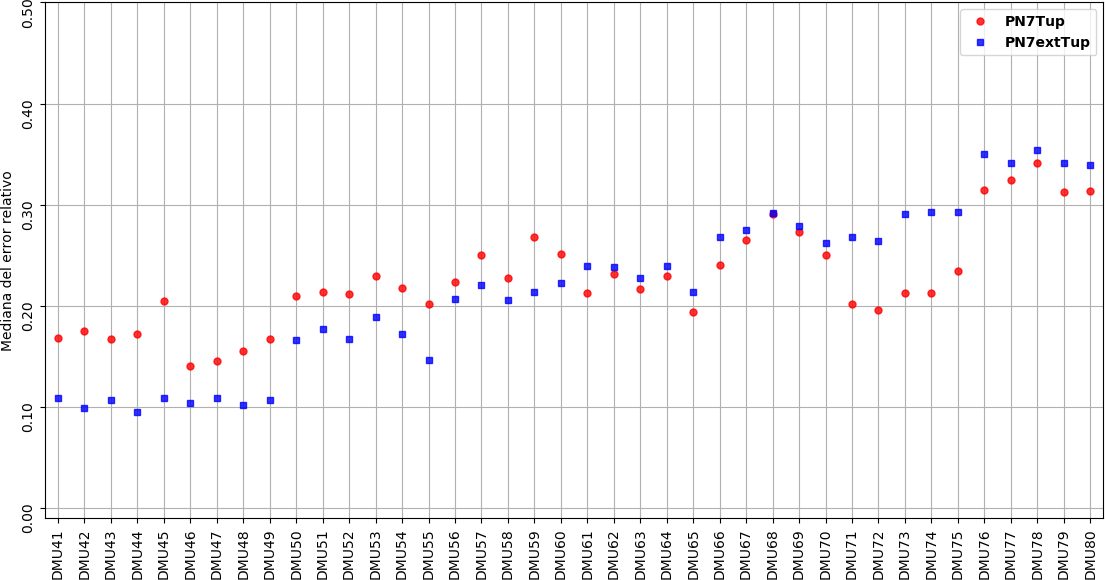
\includegraphics[height=.78\textwidth,width=.95\textheight,angle=270]{Imagenes/n8vsn7err2.png}
        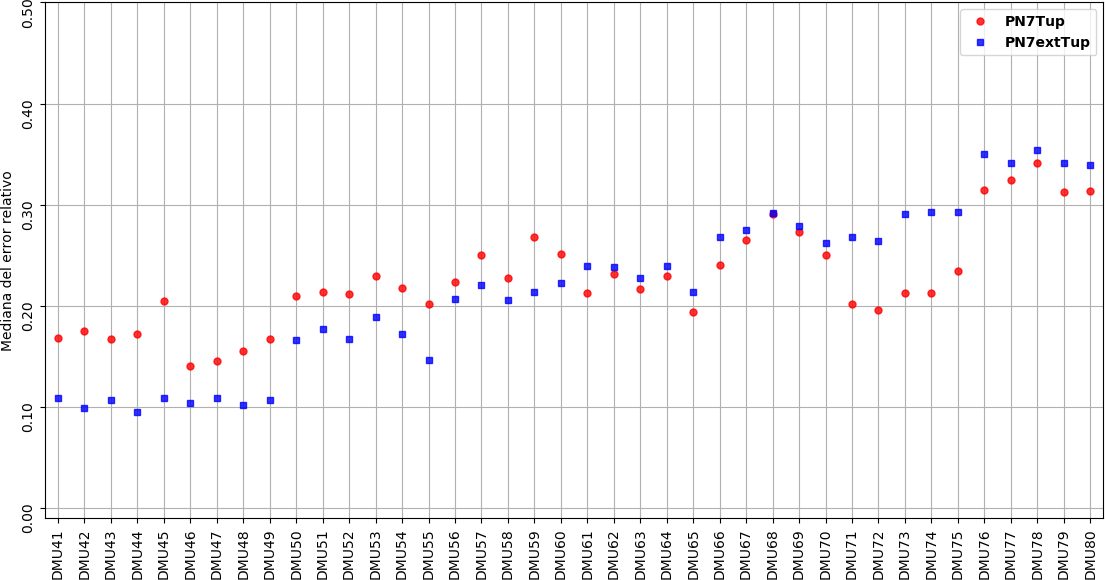
\includegraphics[scale=.6]{Imagenes/n8vsn7err2.png}
        \caption{Resultados para las instancias \textbf{DMU41-80}}
    \end{subfigure}
    \caption{Resultados para ambos métodos. Se marcan los casos en los que se llegó a la mejor solución conocida.}
\end{figure}

\section{Cambio de representación y vecindad}
El cambio de representación y vecindad se compara con las dos propuestas previas. Se sigue el mismo procedimiento mencionado para determinar si hay una diferencia significativa entre los resultados obtenidos.
\begin{figure}[H]
    \centering
    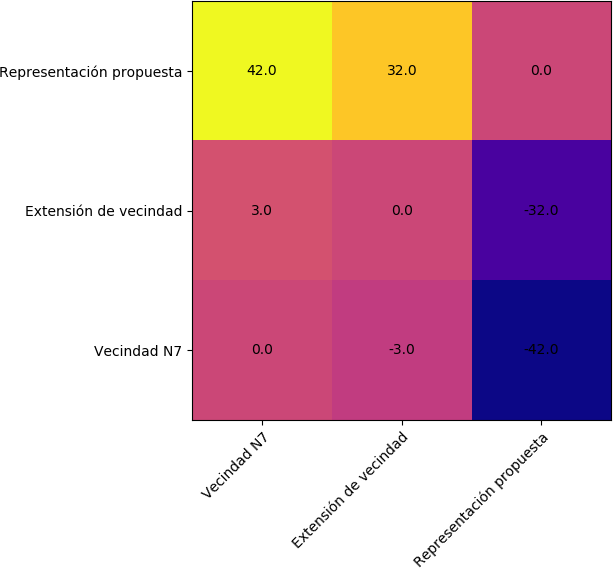
\includegraphics[scale=.7]{Imagenes/prn7n8comp.png}
    \caption{Resultados de la comparación entre los tres métodos.}
\end{figure}
También se muestra la mediana del error relativo alcanzado por los distintos métodos. Los resultados detallados para la extensión de vecindad se encuentran en el apéndice \ref{app:resprtuple}.

\begin{figure}[H]
    \begin{subfigure}{\textwidth}
        \centering
        %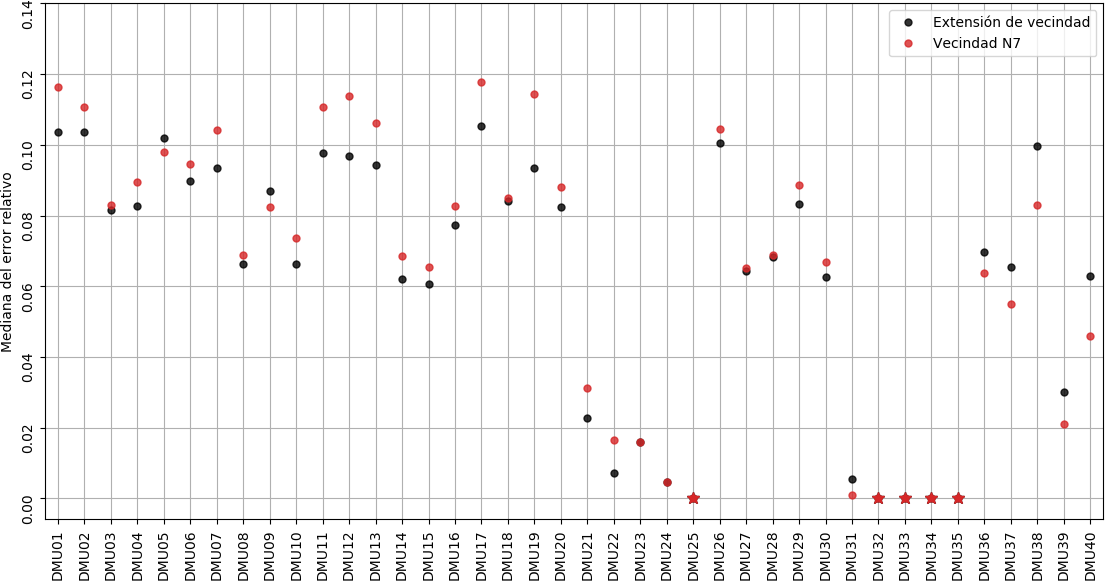
\includegraphics[height=.78\textwidth,width=.95\textheight,angle=270]{Imagenes/n8vsn7err1.png}
        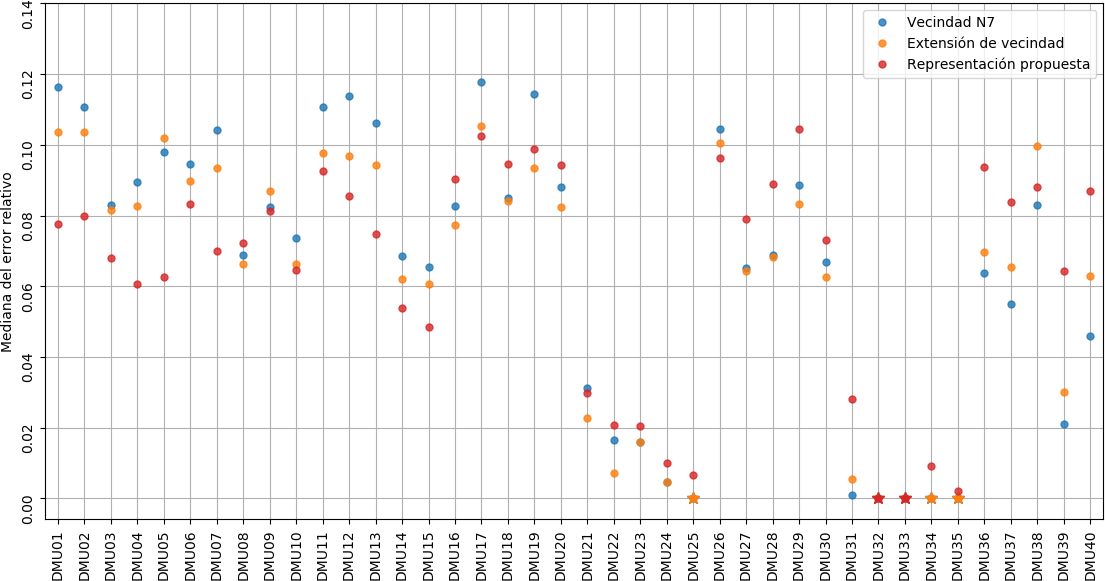
\includegraphics[scale=.6]{Imagenes/prvsn7vsn8err1.png}
        \caption{Resultados para las instancias \textbf{DMU01-40}}
    \end{subfigure}
\end{figure}
\begin{figure}[H]\ContinuedFloat
    \begin{subfigure}{\textwidth}
        \centering
        %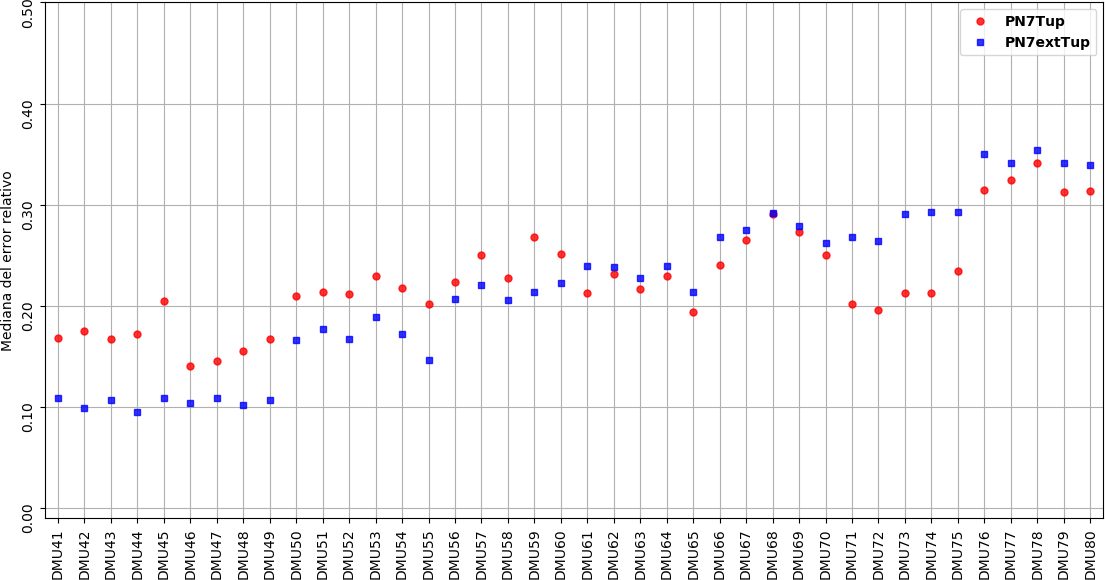
\includegraphics[height=.78\textwidth,width=.95\textheight,angle=270]{Imagenes/n8vsn7err2.png}
        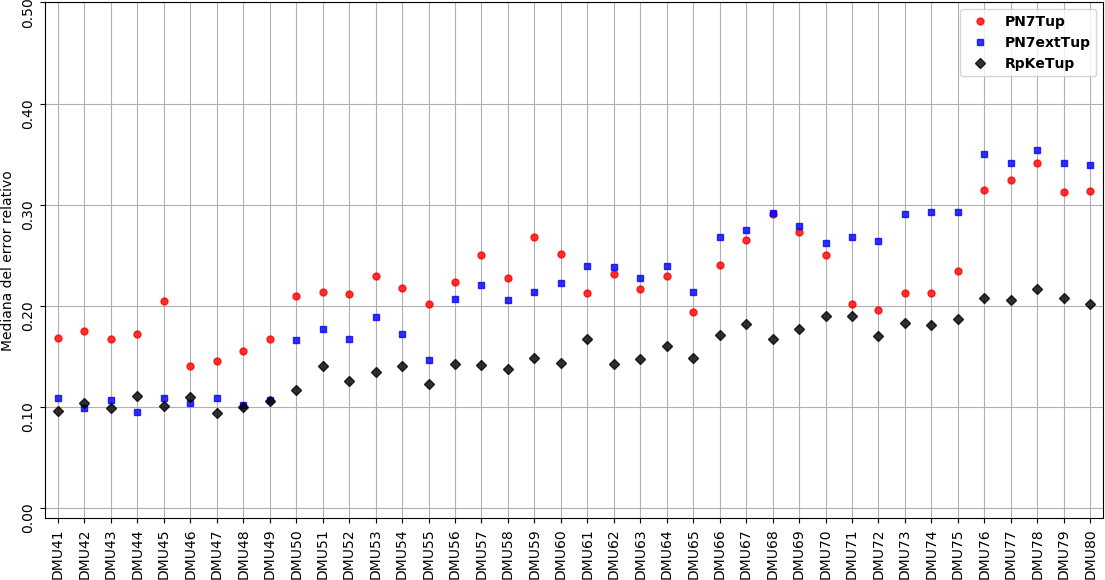
\includegraphics[scale=.6]{Imagenes/prvsn7vsn8err2.png}
        \caption{Resultados para las instancias \textbf{DMU41-80}}
    \end{subfigure}
    \caption{Resultados para ambos métodos. Se marcan los casos en los que se llegó a la mejor solución conocida.}
\end{figure}


Para resaltar las diferencias entre los dos métodos se tomó la instancia en la que se obtuvieron los resultados más dispares, en este caso fue la \textbf{DMU78} y se registró para cada óptimo local visitado su makespan así como el tamaño de su vecindad.

\begin{figure}
    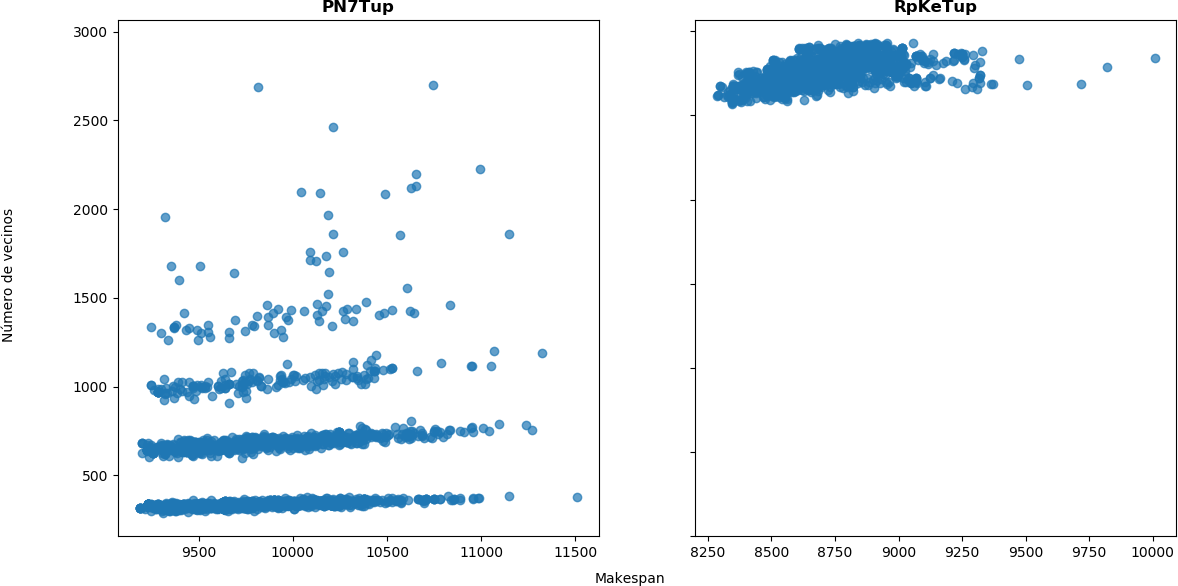
\includegraphics[scale=.6]{Imagenes/compvec78.png}
    \caption{Comparación de tamaño de la vecindad contra makespan de los óptimos locales para la instancia \textbf{DMU78} }
    \label{fig:mattgraph}
\end{figure}
